
%(BEGIN_QUESTION)
% Copyright 2009, Tony R. Kuphaldt, released under the Creative Commons Attribution License (v 1.0)
% This means you may do almost anything with this work of mine, so long as you give me proper credit

Beregn prosentandelen av innkommende effekt som reflekteres tilbake til transmitteren, og prosentandelen av innkommende effekt som blir transmittert (fremover) gjennom væsken i denne radar-nivåmåleapplikasjonen:

$$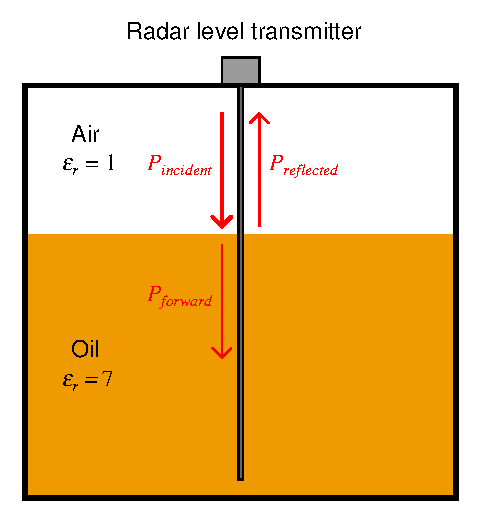
\includegraphics[width=15.5cm]{i00034x01.eps}$$

Beregn også ullage for denne beholderen i fot, gitt en reflektert puls ("echo")-tid på 17.0 nanosekunder.  Anta lyshastighet i vakuum til å være $3 \times 10^8$ meter per sekund.  For alle svar, vis arbeidet ditt!

\vskip 30pt

$P_{reflected}$ = \underbar{\hskip 50pt} \%

\vskip 70pt

$P_{forward}$ = \underbar{\hskip 50pt} \%

\vskip 70pt

Ullage = \underbar{\hskip 50pt} ft

\underbar{file i00034}
%(END_QUESTION)





%(BEGIN_ANSWER)

$P_{reflected}$ = \underbar{\bf 20.38} \%

\vskip 10pt

$P_{forward}$ = \underbar{\bf 79.62} \%

\vskip 10pt

Ullage = \underbar{\bf 8.366} ft

%(END_ANSWER)





%(BEGIN_NOTES)


%INDEX% Measurement, level: radar

%(END_NOTES)
